\newpage 
\appendices

\section{Lineage example}\label{fig:lineage_example}
\begin{figure}[!ht]\label{fig:lineage}
    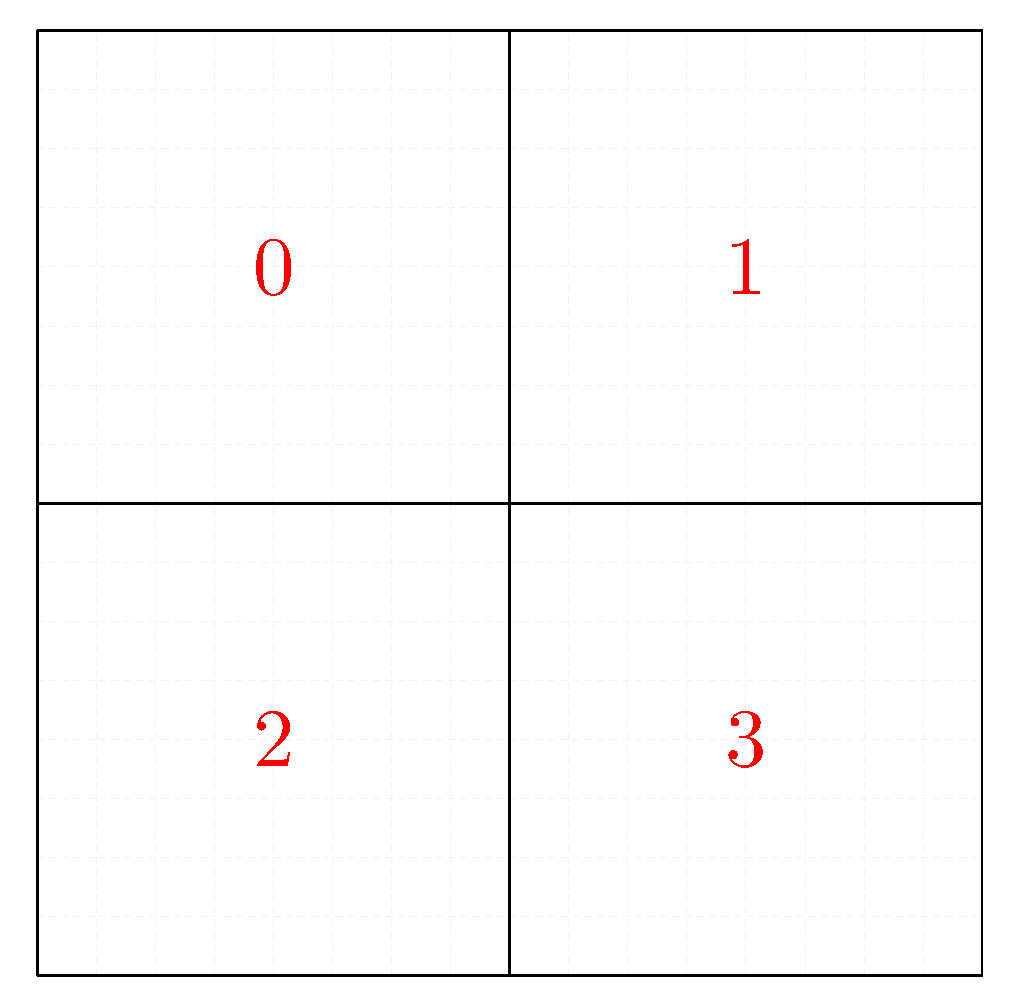
\includegraphics[page=1,width=0.32\linewidth]{figures/cellinpolygon/lineage}
    \includegraphics[page=2,width=0.32\linewidth]{figures/cellinpolygon/lineage}
    \includegraphics[page=3,width=0.32\linewidth]{figures/cellinpolygon/lineage}
    \caption{Lineage can provide the cell's position (string's last character) and its depth (string's length).}
\end{figure}

\section{Empty Cell Algorithm}\label{app:emptycells}
\begin{algorithm} \caption{\textsc{getNextCellWithEdges} algorithm}
    \textbf{Require:} a quadtree with cell envelopes $\mathcal Q$ and map of cells and their edge count $\mathcal M$.
    \begin{algorithmic}[1]
    \Function{ getNextCellWithEdges }{ $\mathcal Q$, $\mathcal M$ }
        \State $\mathcal C \gets $ list of empty cells in $\mathcal M$
        \ForEach{ $emptyCell$ in $\mathcal C $ }
            \State initialize $cellList$ with $emptyCell$ 
            \State $nextCellWithEdges \gets null$
            \State $referenceCorner \gets null$
            \State $done \gets false$
            \While{ not $done$ } 
                \State $c \gets $ last cell in $cellList$ 
                \State $cells, corner \gets \textsc{getCellsAtCorner}(\mathcal Q, c)$ \Comment{ return 3 cells and the reference corner }
                \ForEach{$cell$ in $cells$}
                    \State $nedges \gets$ get edge count of $cell$ in $\mathcal M$ 
                    \If{ $nedges > 0$ }
                        \State $nextCellWithEdges \gets cell$
                        \State $referenceCorner \gets corner$
                        \State $done \gets true$
                    \Else
                        \State add $cell$ to $cellList$
                    \EndIf
                \EndFor
            \EndWhile
            \ForEach{ $cell$ in $cellList$ }
                \State \textbf{output}($cell$, $nextCellWithEdges$, $referenceCorner$)
                \State remove $cell$ from $\mathcal C$
            \EndFor
        \EndFor
    \EndFunction
    \end{algorithmic}
\end{algorithm}

\begin{algorithm} \caption{\textsc{getCellsAtCorner} algorithm}
    \textbf{Require:} a quadtree with cell envelopes $\mathcal Q$ and a cell $c$.
    \begin{algorithmic}[1]
    \Function{ getCellsInCorner }{ $\mathcal Q$, $c$ }
        \State $region \gets $ last character in $c.lineage$
        \Switch{ $region$ }
            \Case{ `0' }
                \State $corner \gets$ left bottom corner of $c.envelope$
            \EndCase
            \Case{ `1' }
                \State $corner \gets$ right bottom corner of $c.envelope$
            \EndCase
            \Case{ `2' }
                \State $corner \gets$ left upper corner of $c.envelope$
            \EndCase
            \Case{ `3' }
                \State $corner \gets$ right upper corner of $c.envelope$
            \EndCase
        \EndSwitch
        \State $cells \gets$ cells which intersect $corner$ in $\mathcal Q$
        \State $cells \gets cells - c$ \Comment{ Remove the current cell from the intersected cells }
        \State $cells \gets$ sort $cells$ on basis of their depth \Comment{ using $cell.lineage$ }
        \State \Return{ ($cells$, $corner$) }
    \EndFunction
    \end{algorithmic}
\end{algorithm}
